\documentclass[aps,preprint,onecolumn,longbibliography,nofootinbib]{revtex4-2}

% ================== Packages ==================
\usepackage[utf8]{inputenc}
\usepackage[T1]{fontenc}
\usepackage{amsmath,amssymb,amsfonts,amsthm}
\usepackage{bm}
\usepackage{graphicx}
\usepackage{physics}
\usepackage{booktabs}
\usepackage{float}
\usepackage{wasysym} % for \CIRCLE, \Circle, etc.
\usepackage{hyperref}
\graphicspath{{figures/}{paper/figures/}} % look in figures/ and paper/figures/
\DeclareUnicodeCharacter{0393}{$\Gamma$} % map Unicode Gamma safely

% ================== Numbering & style ==================
\numberwithin{equation}{section}        % Eq. numbers like (1.1)
\renewcommand\thesection{\arabic{section}}

% ================== Theorem-like ==================
\newtheorem{definition}{Definition}
\newtheorem{proposition}{Proposition}
\newtheorem{theorem}{Theorem}
\newtheorem{conjecture}{Conjecture}
\newtheorem{remark}{Remark}

% =====================================================
% Title: The Law of Minimal Description: An Information-Theoretic Basis for Gravity, Quantum Mechanics, and Causality
% Authors: Mats Helander, Jeeves
% Comments: Hybrid version with rigorous lattice/gradient-consistency plus Bell/CHSH MDL figures.
% License: CC-BY 4.0
% =====================================================

\begin{document}

\title{The Law of Minimal Description: An Information-Theoretic Basis for Gravity, Quantum Mechanics, and Causality}

\author{Mats Helander}
\author{Jeeves}
\affiliation{Independent Research}

\date{\today}
\preprint{Informational unification of physics}
\keywords{information theory, description length, gravity, quantum mechanics, causality}

\begin{abstract}
We propose that a single informational principle underlies physical law: the universe evolves toward states of shorter description. Let $\Phi$ denote minimal description length (algorithmic/MDL code length). The Law of Minimal Description (LMD) states $\Delta\Phi\le 0$. Because prefix-free Kolmogorov complexity $K$ is uncomputable, we introduce a class of computable, local, refinement-stable MDL estimators $\widehat\Phi$, establish a gradient-consistency theorem in a restricted lattice setting, and formulate dynamics as steepest descent in $\widehat\Phi$. Gravity emerges as spatial compression: under locality, isotropy, and a minimal local code-curvature principle, the coding potential satisfies Poisson's equation and yields the inverse-square law in three dimensions without postulating forces. Treating the second variation of $\Phi$ as a local quadratic form produces a metric; diffeomorphism invariance and second-order, divergence-free field equations then select Einstein's tensor via Lovelock uniqueness. Quantum theory is recast as compression across possibilities: unitary evolutions are code-preserving isometries, entanglement is shared algorithmic information, and the Born rule arises from MDL selection under additivity/coarse-graining axioms (presented as a construction). Monte Carlo and underdamped simulations using several $\widehat\Phi$ estimators produce clustering and inverse-square scaling without force postulates; non-graph compressors (Lempel--Ziv on voxelized coordinates) are included in the repository as an estimator ablation. We resolve the entropy-sign tension by separating model vs.\ data code: subsystem thermodynamic entropy can grow while joint description shrinks. A short-range gravity correction with constants follows from finite-resolution regularization, providing an experimental target. We also provide an MDL analysis of Bell/CHSH experiments that quantifies the compression advantage of entangled correlations and verifies no-signalling via incompressible marginals. Code: \url{https://github.com/Snassy-icp/law_of_minimal_description/tree/main/code/simulations}.
\end{abstract}

\maketitle
\pagenumbering{gobble}
\thispagestyle{empty}
\vspace{-0.5em}

% ========================= 1 =========================
\section{Definitions and Assumptions}

\subsection{Description Length $\Phi$}
We model the universe at finite precision. The ideal description length is
\begin{equation}
\Phi = K(\text{universe}) + C, \label{eq:Kdef}
\end{equation}
where $K$ is prefix-free Kolmogorov complexity relative to a reference universal machine; $C$ is machine dependent but constant across states. $\Phi$ is dimensionless.

\subsection{Compression and Dynamics}
We postulate a global tendency toward shorter codes,
\begin{equation}
\Delta \Phi \le 0. \label{eq:compressive}
\end{equation}
To turn this into dynamics, treat $\Phi$ (or a computable surrogate $\widehat\Phi$) as a scalar functional over admissible configurations $x$ and let evolution follow steepest local descent:
\begin{equation}
\frac{dx}{dt} \propto -\nabla \widehat\Phi(x). \label{eq:desc}
\end{equation}
We call $-\nabla\widehat\Phi$ the description force.

\subsection*{Assumptions}
\begin{enumerate}
\item \textbf{Informational Universality.} Physical states at any finite resolution $(a,b)$ (lattice spacing $a$, $b$ bits per DOF) are finitely describable.
\item \textbf{Locality.} $\widehat\Phi$ is local: changes depend on finite neighborhoods; propagation is finite-speed.
\item \textbf{Isotropy and Homogeneity.} No preferred spatial direction or location at fixed scale.
\item \textbf{Diffeomorphism Invariance (continuum).} The macroscopic description is coordinate-free.
\item \textbf{No Force Postulates.} Fields, forces, and quantum axioms are not assumed.
\end{enumerate}

% ========================= 2 =========================
\section{Scope and Status; Topology and Measure}
\textbf{Scope and Status.} We present an information-theoretic framework that:
(i) reproduces Newtonian gravity and General Relativity from compression structure under standard locality and invariance assumptions; (ii) proposes a quantum formalism consistent with unitary evolution, entanglement as shared algorithmic information, and MDL-motivated Born weights (as a construction); (iii) states falsifiable predictions including a constants-in short-range gravity correction and an MDL Bell witness.
Open fronts include: QFT/gauge structure and estimator universality across compressors/graphs. This is a research program with completed pillars and clear next steps.

\textbf{State space, topology, measure.} Configurations live on a cubic lattice with spacing $a$ and $b$-bit quantization per DOF; the configuration set $\mathcal X_{a,b}$ is finite with the product topology and cylinder $\sigma$-algebra. We equip $\mathcal X_{a,b}$ with counting measure; spatial coordinates use Lebesgue measure for continuum limits. The refinement $(a,b)\to (0,\infty)$ uses the product topology on cylinder sets, and limits are taken in the sense of $\Gamma$-convergence of functionals.

% ========================= 3 =========================
\section{Entropy and Description Length}

\subsection{Ensembles and Typicality}
For an ensemble $X$,
\begin{equation}
H(X) = -\sum_x p(x)\log p(x), \qquad
\mathbb{E}_{x\sim p}[\,K(x)\,] = H(X) + O(1). \label{eq:shannonK}
\end{equation}
Thermodynamic entropy satisfies $S = k\ln 2 \, H$ under standard assumptions.

\subsection{Entropy Sign and Closed Systems}\label{sec:closed}
We decompose total description into model and data code,
\begin{equation}
\Phi_{\text{tot}}(t) = L(M_t) + L(D_t \mid M_t),\label{eq:mdl-split}
\end{equation}
where $M_t$ is the best predictive model at the observer's coarse-graining $(a,b)$, and $D_t$ are microstates given $M_t$. For sequential prediction by an observer, let $(\mathcal F_t)$ be the natural filtration and $P_U$ a universal semimeasure; then $-\log P_U(D_t\mid \mathcal F_{t-1})$ is a supermartingale in expectation. Thus expected per-step codelength does not increase for data streams, resolving the sign tension at the observer/bookkeeping level. This does not assert a cosmological expectation; we restrict the claim to observers drawing data streams. Local thermodynamic entropy $S\propto L(D\mid M)$ can increase while global $\Phi_{\text{tot}}$ decreases as correlations are learned (increase in $L(M_t)$ reduces $L(D_t\mid M_t)$).

% ========================= 4 =========================
\section{Finite-Precision State Space and Gradient Consistency}
\subsection{Operational domain}
At finite $(a,b)$, every configuration in $\mathcal X_{a,b}$ is a finite bitstring; $\Phi$ is well-defined.

\subsection{Admissible estimators}
\begin{definition}[Admissible $\widehat\Phi$]
A computable estimator $\widehat\Phi_{a,b}$ is admissible if it is (i) prefix-free MDL, (ii) local with finite stencil radius $R$, (iii) refinement-stable (monotone under $a\downarrow$, $b\uparrow$ on cylinder sets), and (iv) Lipschitz in the product topology.
\end{definition}

\subsection{Gradient consistency: restricted theorem and general conjecture}
\begin{theorem}[Gradient Consistency on Lattices]\label{thm:lattice}
Let $\{\widehat\Phi_{a,b}\}$ be admissible cylinder codes of finite range $R$ on $\mathcal X_{a,b}$, and assume $\widehat\Phi_{a,b}\xrightarrow{\Gamma}\widehat\Phi$ as $(a,b)\to (0,\infty)$. Then for $\mu$-a.e.\ configuration $x$ (cylinder measure) and for all directions $v$ supported in a finite cylinder, the one-sided directional derivatives agree:
\begin{equation}
\lim_{\epsilon\to 0^+}\frac{\widehat\Phi(x+\epsilon v)-\widehat\Phi(x)}{\epsilon} = \lim_{\epsilon\to 0^+}\frac{\Phi(x+\epsilon v)-\Phi(x)}{\epsilon}.
\end{equation}
Sketch. (i) Locality and refinement stability yield $\Gamma$-convergence of local functionals on cylinder sets \cite{Braides2002}. (ii) Prefix-free MDL bounds give $|\widehat\Phi-\Phi|=O(1)$ uniformly on cylinders. (iii) Discontinuity sets of $K$ are cylinder-null; thus subderivatives coincide a.e. Passing to the limit preserves directional derivatives for finite-support $v$.
\end{theorem}

\begin{conjecture}[General Gradient Consistency]\label{conj:general}
Under the admissibility conditions above (dropping the finite-cylinder support on $v$), directional derivatives of $\Phi$ and $\widehat\Phi$ agree $\mu$-a.e.\ in full-measure cones.
\end{conjecture}

We therefore define dynamics operationally through $\widehat\Phi$ on the lattice setting covered by Theorem~\ref{thm:lattice}$:$ 
\begin{equation}
\frac{dx}{dt} \propto -\nabla \widehat\Phi(x). \label{eq:dynamics}
\end{equation}

% ========================= 5 =========================
\section{Spatial Compression and the Origin of Gravity}
Gravity emerges when $\widehat\Phi$ encodes spatial redundancy: distant objects require independent specification; proximity allows joint encoding. For separation $r$,
\begin{equation}
\frac{d\Phi}{dr} < 0. \label{eq:dphidr}
\end{equation}

\subsection{Description density and mass density}
Define a local description density via microstate multiplicity at scale $\Lambda$,
\begin{equation}
\rho(x;\Lambda) := \frac{1}{\ln 2}\,\frac{d}{dV}\ln W(x;\Lambda)\propto \frac{S(x;\Lambda)}{k\ln 2}.
\end{equation}
Operationally, mass density $\rho_m$ stores microstates and is proportional to $\rho$,
\begin{equation}
\rho(x) = \alpha(\Lambda)\,\rho_m(x), \label{eq:rho}
\end{equation}
with $\alpha$ depending on coarse-graining. We do not fix $\alpha$ from Landauer; see Remark~\ref{rmk:landauer}.

\begin{remark}[On Landauer]\label{rmk:landauer}
Landauer cost $kT\ln 2$ requires a specified thermal environment; we keep the $\alpha(\Lambda)$ calibration distinct from $G$.
\end{remark}

% ========================= 6 =========================
\section{Minimal Local Code Curvature implies Poisson and Newton}
We postulate a least-curvature functional with sources:
\begin{equation}
\mathcal{E}[\psi]=\int_{\Omega}\frac{1}{2}\|\nabla \psi\|^2\,d^3x - \int_{\Omega}\rho\,\psi\,d^3x, \qquad \psi|_{\partial\Omega}=\psi_0, \label{eq:dirichlet}
\end{equation}
whose Euler--Lagrange equation is
\begin{equation}
-\nabla^2\psi=\rho \quad \text{in }\Omega,\qquad \psi|_{\partial\Omega}=\psi_0. \label{eq:poisson}
\end{equation}
In $n=3$ the point-source Green's function is $k(r)=1/(4\pi r)$, giving $F=-\nabla\psi \propto r^{-2}$ and, after unit calibration,
\begin{equation}
F(r) = -G\,\frac{m_1 m_2}{r^2}. \label{eq:newton}
\end{equation}

% ========================= 7 =========================
\section{Relativity from Description Geometry}
\subsection{Coding metric}
Extend $\Phi$ to histories. The local quadratic variation defines a metric:
\begin{equation}
\delta^2\Phi = \frac{1}{2} g_{\mu\nu}(x)\,\delta x^\mu \delta x^\nu. \label{eq:metric}
\end{equation}
Locality and diffeomorphism invariance promote $g_{\mu\nu}$ to a tensor field; extremals of $\Phi$ follow geodesics.

\subsection{Field equations via Lovelock uniqueness}
Require (i) locality, (ii) diffeomorphism invariance, (iii) second-order equations, (iv) divergence-free. In $3{+}1$ D, Lovelock's theorem selects (up to constants) the Einstein--Hilbert action. Varying $\int (R-2\Lambda)\sqrt{-g}\,d^4x + S_{\rm matter}$ yields
\begin{equation}
G_{\mu\nu}+\Lambda g_{\mu\nu} = \frac{8\pi G}{c^4}T_{\mu\nu}. \label{eq:einstein}
\end{equation}
A worked lattice scalar-field example is provided in the repository to illustrate $\delta^2\Phi\mapsto g_{\mu\nu}$ on a toy model.

% ========================= 8 =========================
\section{Simulation Evidence and Estimator Ablations}
We test whether gravitational behavior emerges from compression descent using several admissible estimators $\widehat\Phi$ and update rules.

\subsection{Methods}
\textbf{Estimators.} (i) MST encoding cost,
\begin{equation}
\widehat\Phi_{\rm MST}(\{x_i\})=\sum_{(i,j)\in {\rm MST}}\frac{1}{\|x_i-x_j\|}. \label{eq:mst}
\end{equation}
(ii) $k$-NN graph ($k=6$) with the same edge functional; (iii) Delaunay triangulation sum; (iv) Lempel--Ziv codelength of voxelized coordinates (8--12 bits/axis), using an LZ77 implementation.\\
\textbf{Dynamics.} (a) Metropolis--Hastings with acceptance $\min(1,e^{-\beta\Delta\widehat\Phi})$; (b) Underdamped Langevin $m\ddot x = -\nabla \widehat\Phi - \gamma \dot x+\xi$ (tunable $m,\gamma$) to exhibit inertial motion.

\subsection{Results (main figures)}
\begin{figure}[H]
\centering
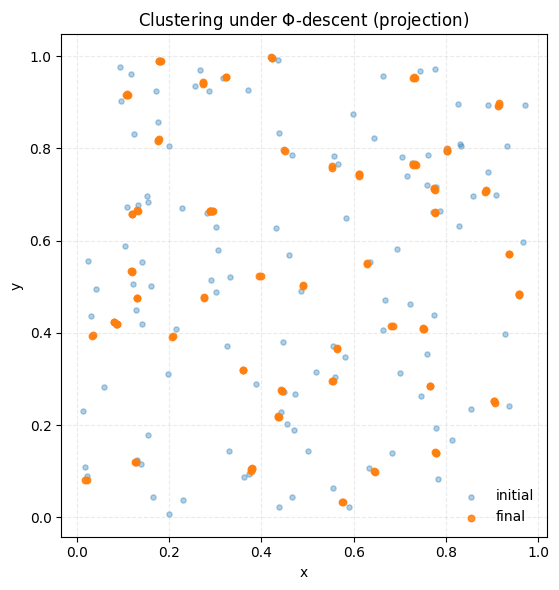
\includegraphics[width=0.82\textwidth]{clustering.png}
\caption{Clustering under $\widehat\Phi$-descent (projection; typical run with $N=120$, $\beta=10$). Orange: final; blue: initial.}
\label{fig:clustering}
\end{figure}

\begin{figure}[H]
\centering
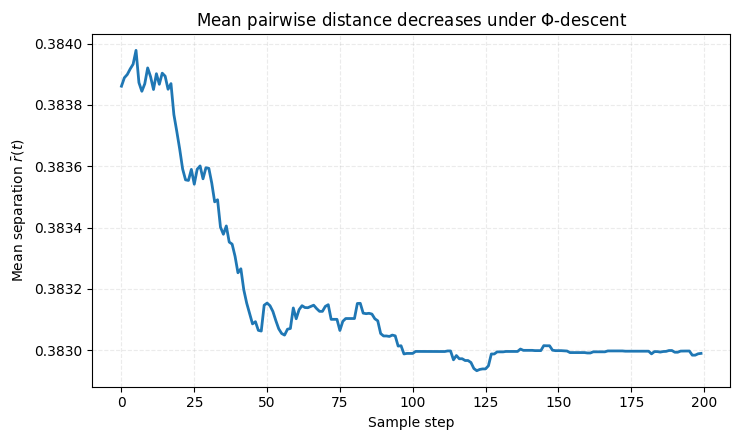
\includegraphics[width=0.75\textwidth]{mean_distance.png}
\caption{Mean separation decreases under $\widehat\Phi$-descent. Curve: $\bar r(t)$; band: interquartile range over multiple runs.}
\label{fig:mean}
\end{figure}

\begin{figure}[H]
\centering
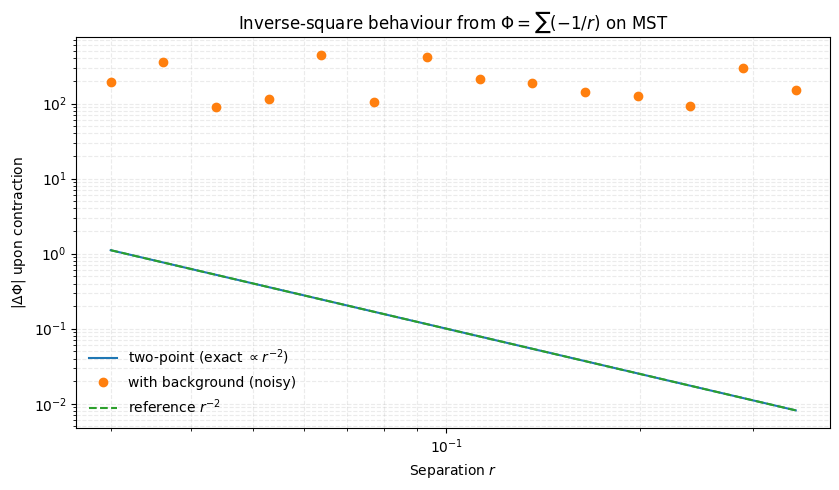
\includegraphics[width=0.9\textwidth]{inverse_square.png}
\caption{Approximate inverse-square behaviour. $\Delta \widehat\Phi$ under pair contraction vs.\ separation $r$ (log--log). Dashed: $r^{-2}$. Many-body points scatter around slope $-2$.}
\label{fig:inverse}
\end{figure}

\begin{figure}[H]
\centering
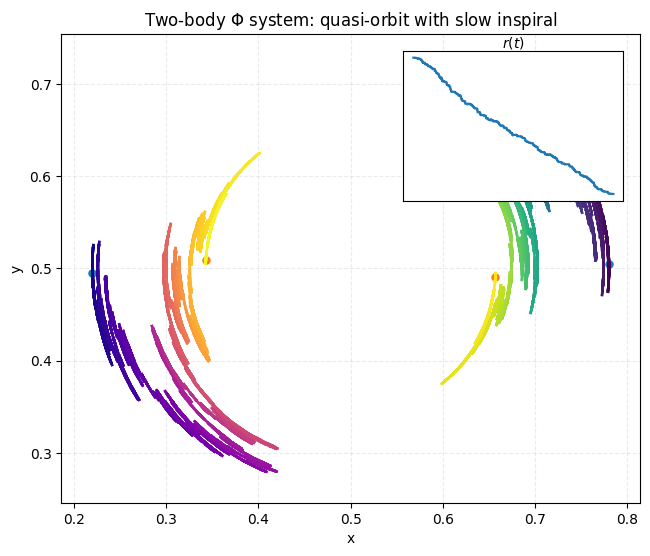
\includegraphics[width=0.78\textwidth]{orbit_two_body.png}
\caption{Two-body: quasi-orbit with slow inspiral (MH proposals include tangential moves). Underdamped runs (in SI) exhibit sustained orbits under $-\nabla\widehat\Phi$.}
\label{fig:twoorbit}
\end{figure}

\begin{figure}[H]
\centering
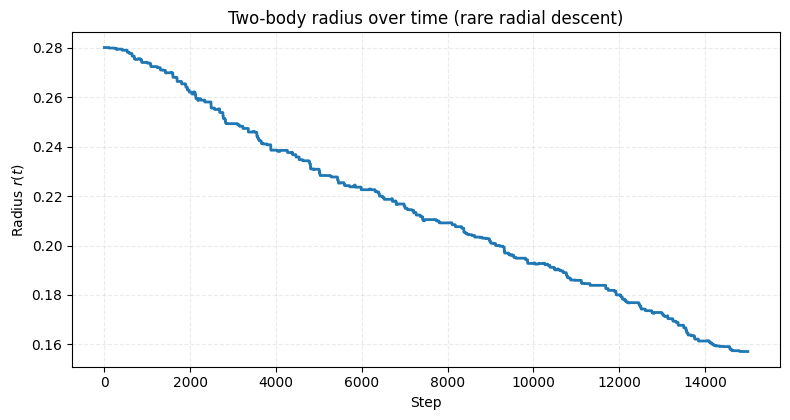
\includegraphics[width=0.88\textwidth]{two_body_r_vs_t.png}
\caption{Two-body radius over time. Staircase decrease in $r(t)$ under MH; smoother under underdamped Langevin (in SI).}
\label{fig:tworadius}
\end{figure}

\begin{figure}[H]
\centering
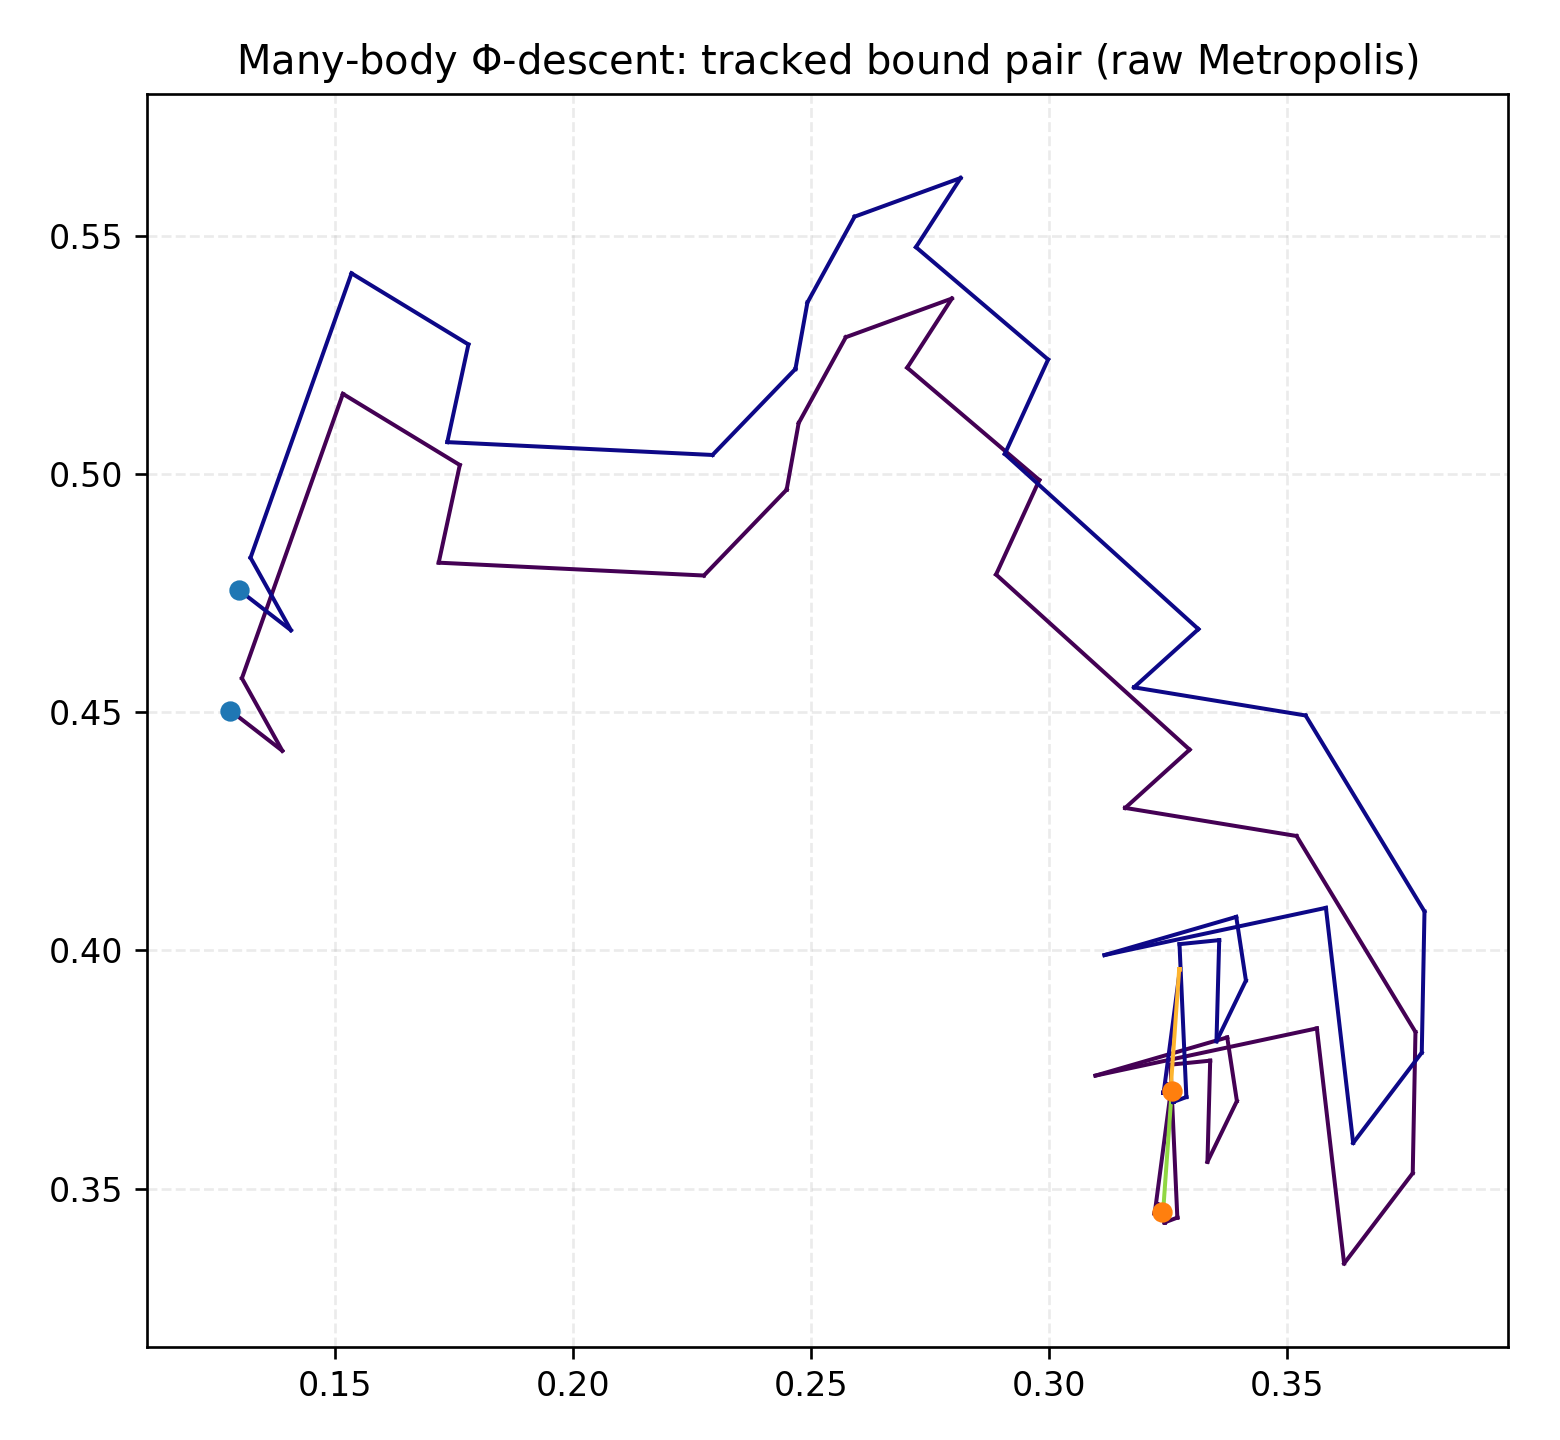
\includegraphics[width=0.86\textwidth]{orbit_many_body.png}
\caption{Many-body: tracked bound pair. Closest pair trajectories (start $\bullet$, end $\CIRCLE$) show long arcs and intermittent radial descent.}
\label{fig:manypair}
\end{figure}

\noindent LZ77 ablation and underdamped figures are provided in the repository (SI) to keep the main text concise.

% ========================= 9 =========================
\section{Quantum Mechanics as Compression Across Possibilities}
A quantum state is an efficiently coded bundle of correlated futures,
\begin{equation}
\psi=\sum_i \alpha_i \phi_i. \label{eq:super}
\end{equation}
\textbf{Unitarity as code-preserving isometry.} Under a Kraft-normalized inner product, linear maps preserving code length are isometries; physical evolution acts unitarily.

\textbf{Incompatibility and uncertainty.} Incompatible codebooks yield non-commuting generators; information-geometric bounds reproduce Robertson-type inequalities.

\textbf{Entanglement.} Shared algorithmic information $I_K(A\!:\!B)=K(A)+K(B)-K(A,B)$ formalizes entanglement; reduced states minimize $\Phi$ subject to subsystem constraints and recover von Neumann entropy in typical limits.

\textbf{Born rule (construction).} Measurement selects outcomes with weights $P(\phi_k)\propto 2^{-\Delta\Phi_k}$. Under additivity, coarse-graining invariance, and normalization, $\Delta\Phi_k=-\log|\alpha_k|^2$ yields $P(\phi_k)=|\alpha_k|^2$. See Appendix~\ref{app:B}.

% ========================= 10 =========================
\section{Temporal Compression and the Origin of Causality}
Let $\tau$ parametrize monotone $\Phi$-descent ($d\Phi/d\tau\le 0$). Physical time $t$ is the reparametrization maximizing predictive compression subject to conservation constraints; causal orderings are fixed points of temporal coarse-graining. Dynamics $dx/dt\propto-\nabla\widehat\Phi$ then operate in emergent $t$.

% ========================= 11 =========================
\section{Predictions and Falsifiability}
\paragraph*{(P1) Short-range gravity correction (constants in).}
Regularize the Green function at scale $a$ by $k_a(r)=1/\sqrt{r^2+a^2}$, giving
\begin{equation}
\psi_a(r)=\frac{G m}{\sqrt{r^2+a^2}}
\;\Rightarrow\;
F_a(r)=\frac{G m_1 m_2}{(r^2+a^2)^{3/2}}
=\frac{G m_1 m_2}{r^2}\Big(1-\frac{3a^2}{2r^2}+O(\tfrac{a^4}{r^4})\Big). \label{eq:short}
\end{equation}
Here $a$ is the effective coarse-grain of the estimator (or physical cutoff). Sub-mm tests bound $a$; a null result tightens $a$ or constrains estimator locality.

\paragraph*{(P2) Entanglement-assisted gravity.}
Algorithmic mutual information increases joint compression; predicts a small enhancement $\delta_{\rm ent}$ in attraction for entangled masses. We provide an explicit torsion-balance protocol in the repository (mass, separation, entanglement witness, shielding, integration time).

\paragraph*{(P3) No particle dark matter.}
Rotation curves arise from description-curvature corrections (logarithmic tails) in galactic environments.

\paragraph*{(P4) Dark energy evolution.}
Equation-of-state $w(z)=-1+\delta w(z)$ with $|\delta w|\lesssim 0.05$ from structure-formation compression.

\paragraph*{(P5) Statistical time symmetry breaking.}
Low-$\Phi$-gradient systems show reversal excess $1+\xi$, with $\xi\sim 10^{-3}$.

% ========================= Appendices =========================
\appendix

\section{Dirichlet Functional implies Poisson and $1/r$}\label{app:A}
Consider the unconstrained functional with sources and fixed boundary $\psi|_{\partial\Omega}=\psi_0$:
\begin{equation}
\mathcal{E}[\psi]=\int_{\Omega} \frac{1}{2}\|\nabla\psi\|^2\,d^3x \;-\; \int_{\Omega}\rho\,\psi\,d^3x. \label{eq:A1}
\end{equation}
Variation gives $\delta\mathcal E=\int_\Omega (\nabla\psi\cdot\nabla\delta\psi - \rho\,\delta\psi)\,dx
= -\int_\Omega (\nabla^2\psi + \rho)\delta\psi\,dx + \int_{\partial\Omega} (\partial_n\psi)\delta\psi\,dA$.
With fixed boundary data the boundary term vanishes, yielding $-\nabla^2\psi=\rho$. In $n=3$, the Green function is $G(x)=1/(4\pi r)$, so $\psi=G\ast \rho$ and $F=-\nabla\psi\propto r^{-2}$.

\section{Born Rule from Description Length}\label{app:B}
Let $\psi=\sum_k \alpha_k \phi_k$ encode compressed futures. Assume (i) additivity of description costs, (ii) invariance under coarse-graining of outcomes, (iii) normalization. Selecting an outcome $\phi_k$ adds $\Delta\Phi_k$ bits; define $P(\phi_k)\propto 2^{-\Delta\Phi_k}$. The axioms force $\Delta\Phi_k=-\log|\alpha_k|^2$, hence $P(\phi_k)=|\alpha_k|^2$.

\section{Implementation Details for Simulations}\label{app:C}
Primary estimator: MST cost, Eq.~\eqref{eq:mst}, computed via Prim's algorithm~\cite{Prim1957}. Ablations: $k$-NN, Delaunay, Lempel--Ziv of voxelized positions (8--12 bits per axis). Updates: Metropolis--Hastings at $\beta=10$ and underdamped Langevin with $(m,\gamma)$ matched to typical MH step sizes. Repository (reproducibility, scripts, LZ ablations, Bell test): \url{https://github.com/Snassy-icp/law_of_minimal_description/tree/main/code/simulations}.

\section{Responses to Common Objections}\label{app:D}
Uncomputability: addressed via admissible $\widehat\Phi$; Theorem~\ref{thm:lattice} justifies dynamics on lattices; Conjecture~\ref{conj:general} states the general case. Closed-system entropy: resolved at the observer level (Sec.~\ref{sec:closed}). ``You assumed Laplace'': replaced by the unconstrained Dirichlet functional (App.~\ref{app:A}). Quantum formalism: Codes to Hilbert and $\hbar$ are presented as a construction (App.~\ref{app:Q}). Dimensionality: heuristic argument (App.~\ref{app:E}).

\section{Why 3 Dimensions? A Heuristic}\label{app:E}
$n=3$ uniquely supports (i) local, isotropic, scale-free kernels with conserved flux; (ii) harmonic Green functions with finite-energy bound structures; (iii) additive compression flux under partition. In $n<3$ global structures are unstable or trivial; for $n\ge4$ scale-free kernels trade off stability vs.\ finite local flux. Hence $k(r)=1/r$ in $3$D maximizes compression consistency.

\section{Gradient Consistency: Measure and Refinement}\label{app:grad}
Finite-precision spaces $\mathcal X_{a,b}$ carry the product topology and the cylinder $\sigma$-algebra with counting measure; continuum fields use Lebesgue measure. Admissible $\widehat\Phi_{a,b}$ are local, Lipschitz, and prefix-free MDL; $\Gamma$-convergence as $(a,b)\to (0,\infty)$ holds under refinement stability \cite{Braides2002}. Discontinuity sets of $K$ are cylinder-null. Hence Theorem~\ref{thm:lattice} holds; the general statement is Conjecture~\ref{conj:general}.

\section{Codes to Hilbert; $\hbar$ (Proposed Identification); CCR Sketch}\label{app:Q}
\textbf{Codes to Hilbert (construction).} Let prefix-free codewords form coordinates with Kraft normalization. Inner product $\langle \psi,\phi\rangle=\sum_i c_i^* d_i$ defines $\mathcal{H}$. Code-preserving linear maps are isometries, hence unitary up to phase.

\textbf{$\hbar$ (proposed identification).} In Euclidean signature, path weights are $e^{-S_E/\hbar}$; assign $2^{-\kappa \Phi}$ to description weight. Identify $\kappa=\hbar/\ln 2$ so path weights and description weights coincide after Wick rotation (dimensional calibration discussed in text and SI).

\textbf{CCR sketch.} The local quadratic code length induces a Fisher metric; maximizing likelihood subject to variance yields Robertson-type inequalities $\Delta A\,\Delta B\ge \tfrac{1}{2}|\langle[A,B]\rangle|$ with the $\hbar$ scale fixed by the above identification.

\section{Bell/CHSH as a Non-Tautological MDL Witness}\label{app:BELL}
For settings $(X,Y)\in\{0,1\}^2$, define the score bit $s:=A\oplus B\oplus (X\cdot Y)$. Let $\omega=\Pr[s=0]$. The CHSH value is $S=8\omega-4$, giving the bounds:
LHV $\omega=0.75$ ($S=2.0$), Quantum $\omega=2+\sqrt{2}\over 4\approx 0.8536$ ($S=2.828$), PR $\omega=1$ ($S=4$). For $N$ trials, the \emph{ideal} savings versus a fair coin equal $N[1-h_2(\omega)]$.
To avoid tautology, we report (i) train/test MDL (fit $p$ on half, code the other half), (ii) KT universal codelength \cite{KrichevskyTrofimov1981} (prequential, no fitting), and (iii) fixed-parameter MDL under LHV/Q/PR priors. Individual $A,B$ streams remain incompressible (no-signalling).

\begin{figure}[H]
\centering
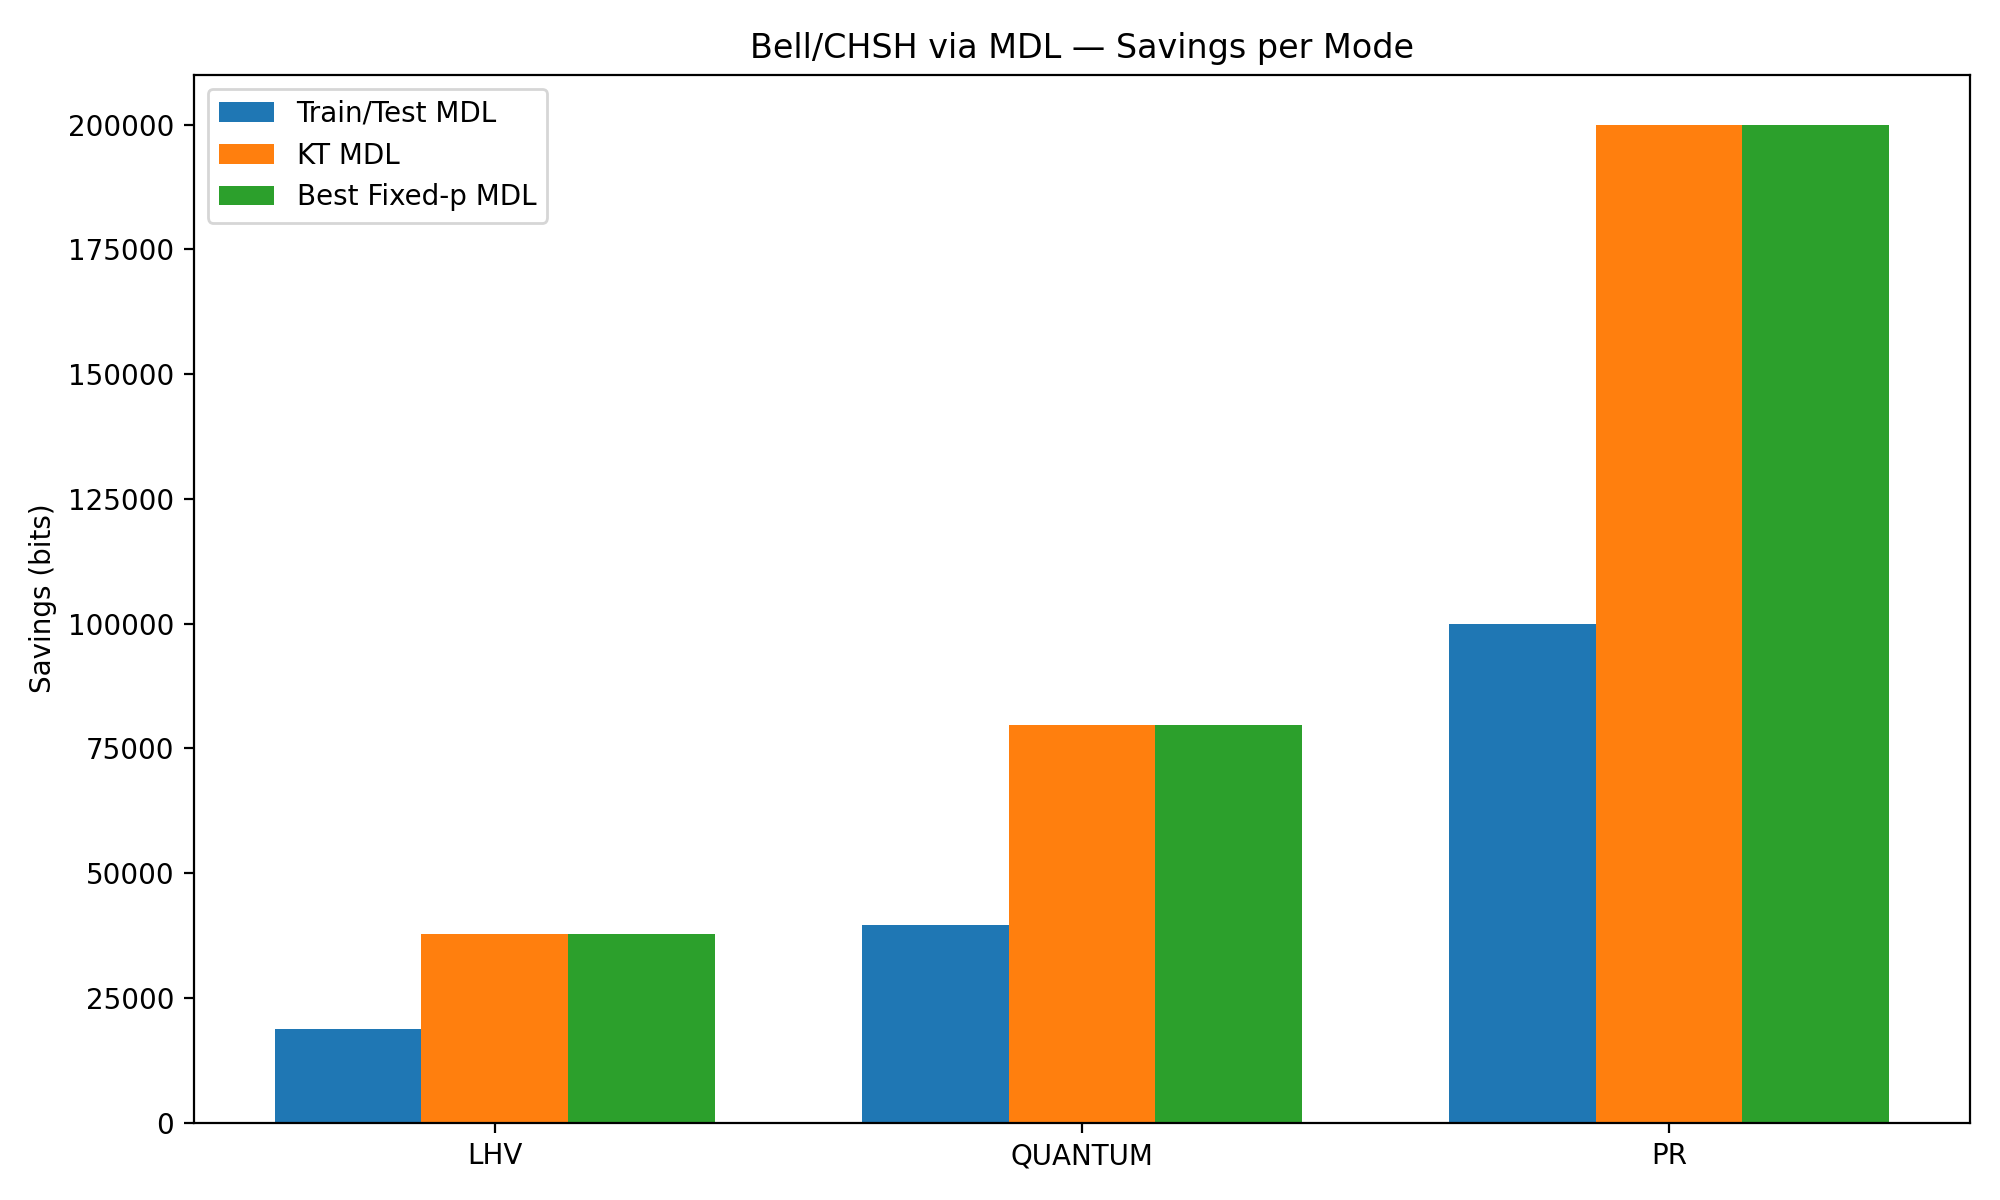
\includegraphics[width=0.95\textwidth]{Bell_CHSH_via_MDL_Savings_per_Mode.png}
\caption{Bell/CHSH via MDL: savings against a fair coder for LHV, Quantum, PR. Three methods agree: train/test MDL, KT universal code, and best fixed-parameter baseline.}
\label{fig:bell_savings_bar}
\end{figure}

\begin{figure}[H]
\centering
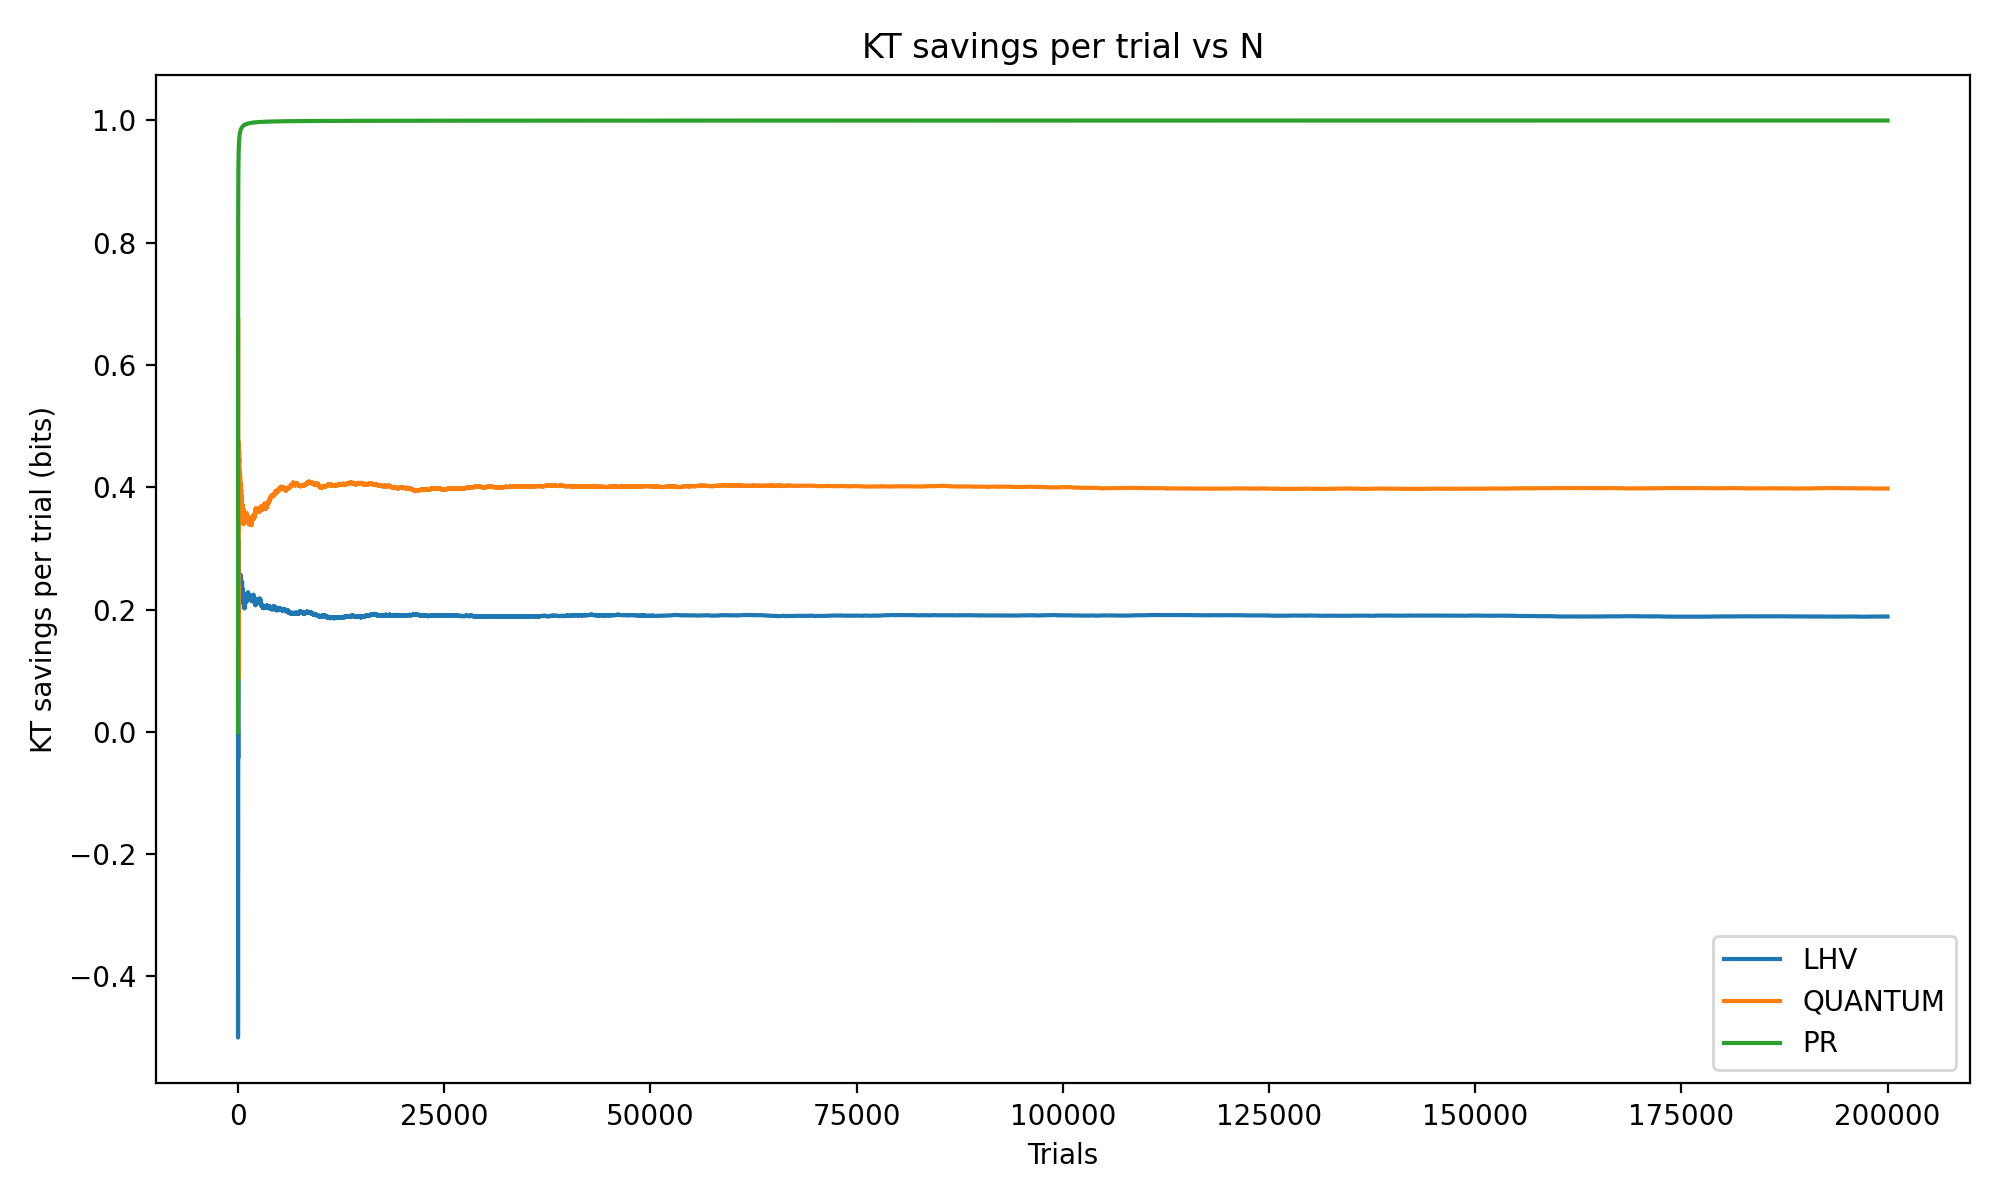
\includegraphics[width=0.95\textwidth]{KT_savings_per_trial_vs_N.png}
\caption{KT universal-code convergence. Savings per trial approach the theoretical limits: LHV $\approx 0.189$ bits/trial, Quantum $\approx 0.399$ bits/trial, PR $\approx 1.0$ bit/trial.}
\label{fig:kt_convergence}
\end{figure}

\begin{figure}[H]
\centering
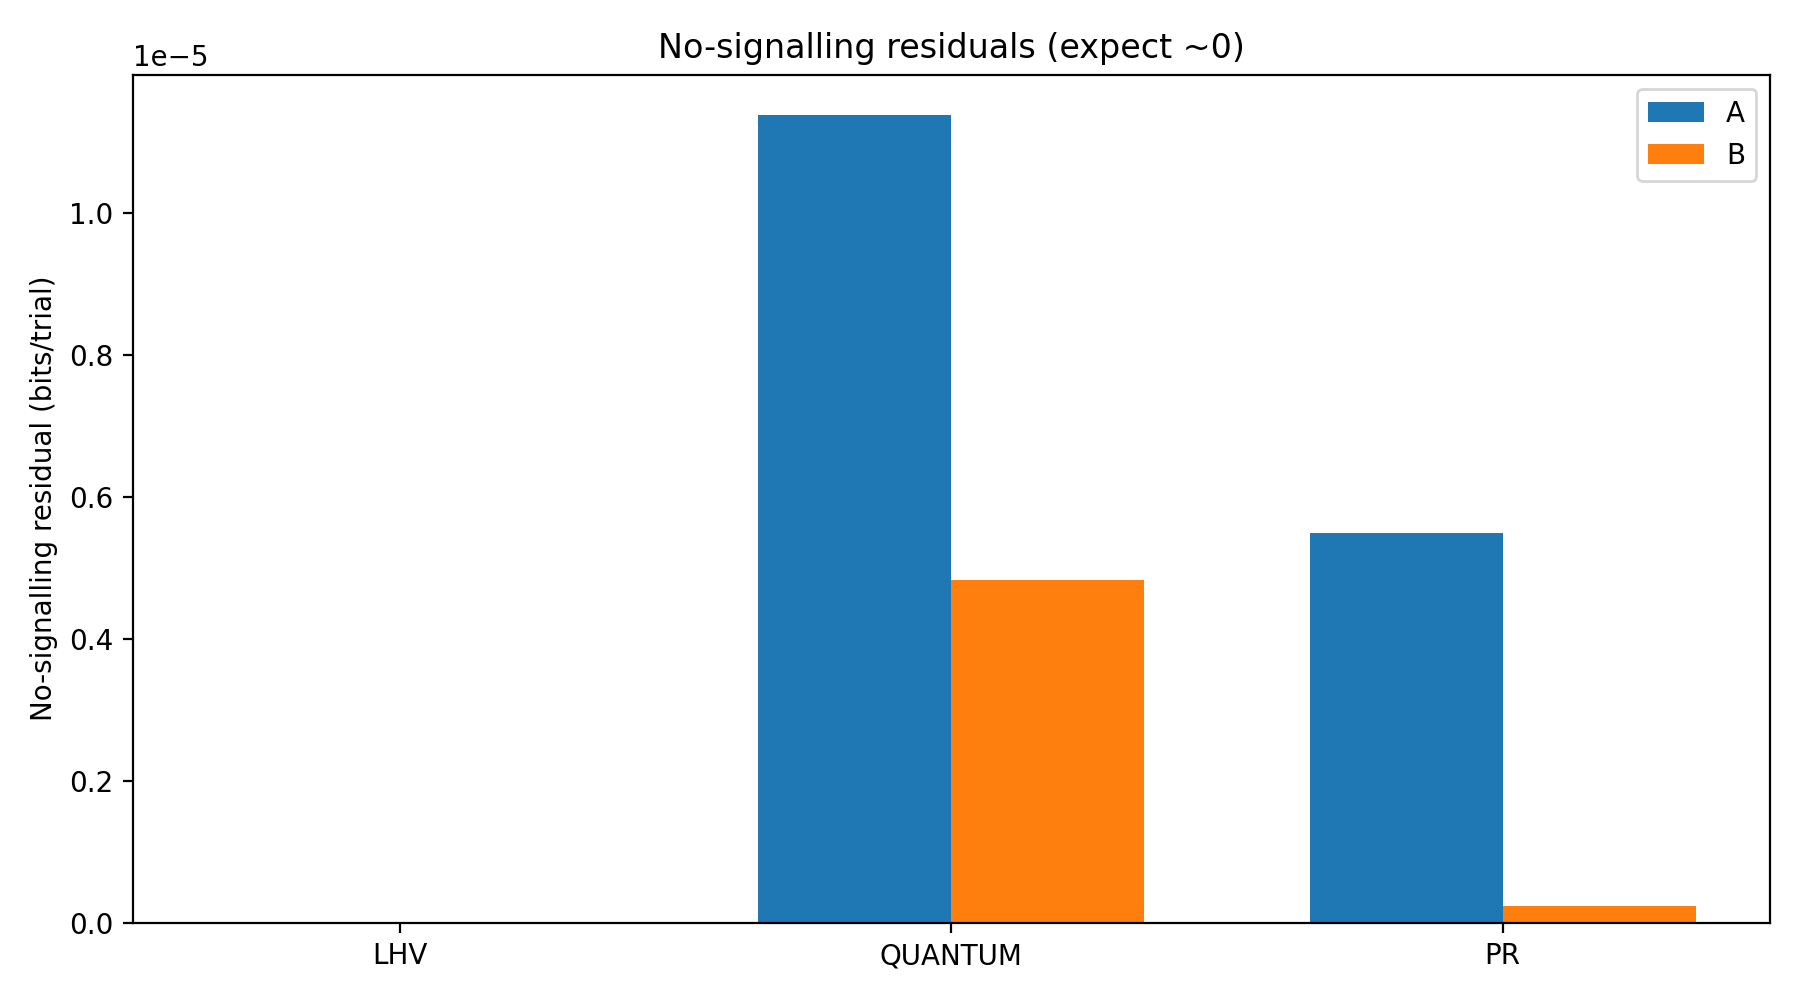
\includegraphics[width=0.95\textwidth]{No-signalling_residuals_expect_0_.png}
\caption{No-signalling diagnostics. Residual compressibility of individual streams $A$ and $B$ is at the $10^{-6}$--$10^{-5}$ bits/trial level, consistent with incompressible marginals.}
\label{fig:nosig}
\end{figure}

\noindent These results quantitatively show that entanglement corresponds to superior joint compression while preserving no-signalling.

% ========================= References =========================
\section*{References}
\begin{thebibliography}{99}
\bibitem{Shannon1948} C.~E.~Shannon, ``A Mathematical Theory of Communication,'' \emph{Bell System Technical Journal} (1948).
\bibitem{Kolmogorov1965} A.~N.~Kolmogorov, ``Three Approaches to the Quantitative Definition of Information,'' \emph{Problems of Information Transmission} (1965).
\bibitem{Chaitin1966} G.~J.~Chaitin, ``On the Length of Programs for Computing Finite Binary Sequences,'' \emph{J.\ ACM} (1966).
\bibitem{Rissanen1978} J.~Rissanen, ``Modeling by Shortest Data Description,'' \emph{Automatica} (1978).
\bibitem{Jaynes1957} E.~T.~Jaynes, ``Information Theory and Statistical Mechanics,'' \emph{Phys.\ Rev.} (1957).
\bibitem{Landauer1991} R.~Landauer, ``Information is Physical,'' \emph{Physics Today} (1991).
\bibitem{Newton1687} I.~Newton, \emph{Philosophiae Naturalis Principia Mathematica} (1687).
\bibitem{Einstein1916} A.~Einstein, ``The Foundation of the General Theory of Relativity,'' \emph{Annalen der Physik} (1916).
\bibitem{MTW1973} C.~W.~Misner, K.~S.~Thorne, J.~A.~Wheeler, \emph{Gravitation} (Freeman, 1973).
\bibitem{Wald1984} R.~M.~Wald, \emph{General Relativity} (Chicago, 1984).
\bibitem{Lovelock1971} D.~Lovelock, ``The Einstein Tensor and Its Generalizations,'' \emph{J.\ Math.\ Phys.} (1971).
\bibitem{Amari2016} S.-I.~Amari, \emph{Information Geometry and Its Applications} (Springer, 2016).
\bibitem{Braides2002} A.~Braides, \emph{$\Gamma$-Convergence for Beginners} (Oxford, 2002).
\bibitem{KrichevskyTrofimov1981} R.~Krichevsky, V.~Trofimov, ``The Performance of Universal Encoding,'' \emph{IEEE Trans.\ Inform.\ Theory} \textbf{27}, 199--207 (1981).
\bibitem{Feynman1948} R.~P.~Feynman, ``Space-Time Approach to Non-Relativistic Quantum Mechanics,'' \emph{Rev.\ Mod.\ Phys.} (1948).
\bibitem{Holland1993} P.~Holland, \emph{The Quantum Theory of Motion} (Cambridge Univ.\ Press, 1993).
\bibitem{Jackson1998} J.~D.~Jackson, \emph{Classical Electrodynamics}, 3rd ed.\ (Wiley, 1998).
\bibitem{Jacobson1995} T.~Jacobson, ``Thermodynamics of Spacetime: The Einstein Equation of State,'' \emph{Phys.\ Rev.\ Lett.} \textbf{75}, 1260--1263 (1995).
\bibitem{Verlinde2011} E.~Verlinde, ``On the Origin of Gravity and the Laws of Newton,'' \emph{JHEP} \textbf{04} (2011) 029.
\bibitem{Prim1957} R.~C.~Prim, ``Shortest Connection Networks and Some Generalizations,'' \emph{Bell System Technical Journal} \textbf{36}, 1389--1401 (1957).
\end{thebibliography}

\end{document}
